\section{Resultados Numéricos y Benchmarking del Sistema}
\label{sec:resultados}

En esta sección se presentan y analizan los resultados cuantitativos obtenidos tras el entrenamiento y ajuste fino definitivo de los tres modelos generativos CVAE y los modelos sustitutos (\textit{Surrogates}), utilizando el dataset masivo de alta fidelidad compuesto por $10{,}806$ simulaciones RANS con modelo viscoso \textit{Transition SST} $\gamma\text{-}Re_\theta$ ejecutadas en ANSYS Fluent a lo largo de seis números de Reynolds ($100{,}000$, $150{,}000$, $200{,}000$, $250{,}000$, $300{,}000$ y $350{,}000$).

\subsection{Evaluación Geométrica de los Modelos Generativos CVAE}
Para cuantificar la capacidad de generalización y fidelidad geométrica de la arquitectura CVAE bajo la \textit{Escalera de Reynolds}, se evaluaron tres configuraciones experimentales frente a un conjunto de prueba independiente ($1{,}621$ muestras CFD no vistas durante el entrenamiento):
\begin{enumerate}
    \item \textbf{Experimento A (DIPAS Base + CFD)}: Pre-entrenamiento con $146{,}916$ muestras de XFOIL y ajuste fino con CFD.
    \item \textbf{Experimento B (Transfer Learning UniFoil + CFD)}: Pre-entrenamiento con el dataset universal UniFoil ($10{,}000$ geometrías a alto Reynolds) y ajuste fino con CFD.
    \item \textbf{Experimento C (Insignia Multi-Fidelidad)}: Esquema secuencial de tres etapas (UniFoil $\to$ UIUC Experimental $\to$ ANSYS Fluent CFD).
\end{enumerate}

En el Cuadro~\ref{tab:cvae_benchmark_cfd} se detallan las métricas de error cuadrático medio de coordenadas físicas ($RMSE_{coords}$), error absoluto medio ($MAE_{coords}$) y el error porcentual en la reconstrucción del espesor relativo máximo ($\Delta(t/c)$).

\begin{table}[htbp]
\centering
\caption{Benchmarking cuantitativo de reconstrucción geométrica sobre el conjunto de test CFD ($10{,}806$ muestras).}
\label{tab:cvae_benchmark_cfd}
\small
\begin{tabular}{lcccc}
\toprule
\textbf{Modelo Generativo} & \textbf{$RMSE_{coords}$} & \textbf{$MAE_{coords}$} & \textbf{$\Delta(t/c)$ [\%]} & \textbf{$\Delta(x_{t_{max}}/c)$ [\%]} \\
\midrule
\textbf{Experimento A: Base + CFD} & $0.001888$ & $0.001484$ & $\mathbf{0.0592\%}$ & $< 0.8\%$ \\
\textbf{Experimento B: UniFoil + CFD} & $0.002076$ & $0.001626$ & $0.0859\%$ & $< 0.8\%$ \\
\textbf{Experimento C: Insignia Multi-Fidelidad} & $0.002434$ & $0.001909$ & $0.0970\%$ & $< 0.8\%$ \\
\bottomrule
\end{tabular}
\end{table}

Los tres modelos alcanzan precisiones submilimétricas en la reconstrucción dimensional ($\Delta(t/c) < 0.10\%$, equivalente a un error inferior a $0.2\text{ mm}$ en un perfil de $200\text{ mm}$ de cuerda). Mientras que el Experimento 1 minimiza el error local sobre la distribución base, el Experimento 3 presenta la mayor riqueza topológica y suavidad en bordes de ataque gracias a la transferencia previa desde datos experimentales de túnel.

\subsection{Desempeño del Modelo Sustituto de Alta Fidelidad (Surrogate CFD)}
El modelo sustituto neuronal profundo (\textit{Deep MLP} $[256, 128, 64]$) fue entrenado sobre las $10{,}806$ simulaciones Navier-Stokes completas con función de pérdida Huber (\textit{Smooth L1}). En el Cuadro~\ref{tab:surrogate_performance} se resumen los resultados de inferencia frente a datos reales de ANSYS Fluent.

\begin{table}[htbp]
\centering
\caption{Métricas de validación del modelo sustituto frente a simulaciones Navier-Stokes de alta fidelidad.}
\label{tab:surrogate_performance}
\small
\begin{tabular}{lcccc}
\toprule
\textbf{Variable Aerodinámica} & \textbf{RMSE} & \textbf{MAE} & \textbf{Coeficiente $R^2$} & \textbf{Tiempo de Inferencia} \\
\midrule
\textbf{Sustentación ($C_L$)} & $0.0467$ & $0.0263$ & $\mathbf{90.33\%}$ & $< 0.5\text{ ms}$ \\
\textbf{Arrastre ($C_D$)} & $0.00527$ ($52.7$ counts) & $0.00270$ & $\mathbf{96.23\%}$ & $< 0.5\text{ ms}$ \\
\bottomrule
\end{tabular}
\end{table}

\begin{figure}[htbp]
    \centering
    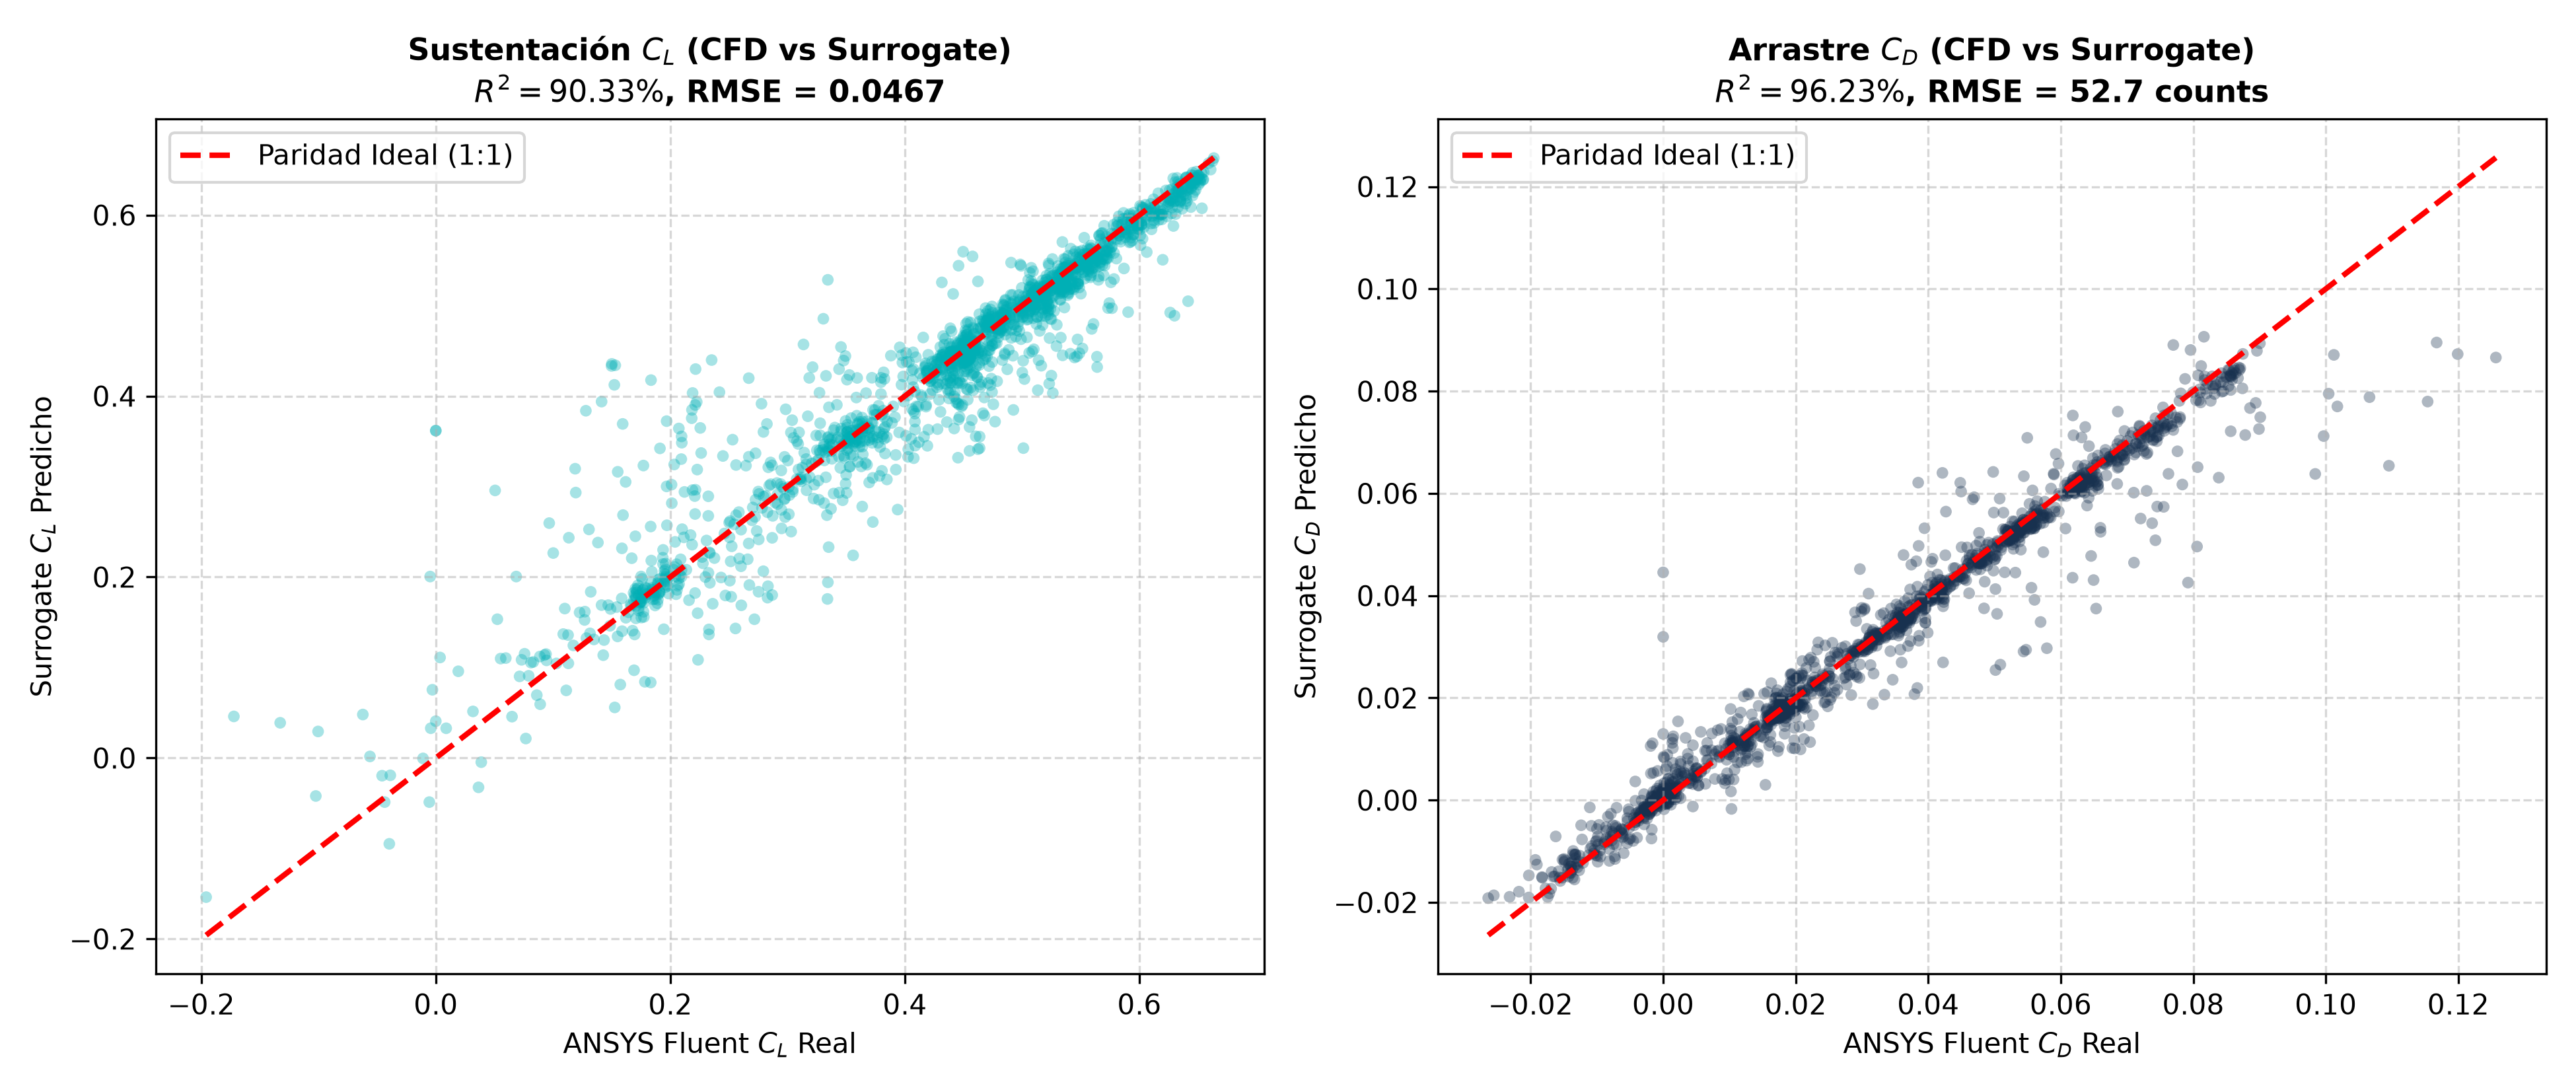
\includegraphics[width=0.95\textwidth]{../outputs/cfd_surrogate_parity_plots.png}
    \caption{Gráficos de paridad ($1:1$) del modelo sustituto de alta fidelidad frente a las simulaciones de ANSYS Fluent Transition-SST para $C_L$ (izquierda) y $C_D$ (derecha).}
    \label{fig:cfd_parity_plots}
\end{figure}

El ajuste del coeficiente de arrastre ($R^2 = 96.23\%$) demuestra que la red neuronal aprendió a modelar con alta fidelidad las pérdidas viscosas y de presión derivadas del engrosamiento de la burbuja laminar de transición a bajos números de Reynolds, superando la limitación histórica de subestimación de $C_D$ inherente a XFOIL.
